\section{Methodology}
\label{sec:methodology}
% Focus on what you add to the existing method. Explain what you will do and why (and how). Do not forget to characterize your research design. There should be a sub-section on the evaluation. 
%For DS students, this normally means using manually labelled or ground truth data. 
% Write about your methodology here. Focus on your own contribution. Indicate exactly how you will assess your work in terms of evaluation.
% It is possible to use a separate section for the Experimental Setup, which then focuses on all settings used in your experiments. It also possible to address the settings in a sub-section under Methodology. 

The goal of the study is to understand the characteristics of storefront signage in relation to gentrification, via learning the font types, colors, and semantics present. The approach that this study takes comprises of multiple models: scene-text detection, scene-text recognition, color histogram, font recognition, word embedding, and gradient boosting. This is because the state-of-the-art is that there has not been a model that takes an interest in analyzing scene-text in a comprehensive manner - much of the focus is on detecting [CITE] and recognizing [CITE] text in the wild with better accuracy. Elements such as fonts and colors are only of interest in the domain of graphic design [CITE]. Therefore, this research serves as a pilot case in utilizing these individual models for feature extraction via transfer learning, and subsequently test these features by using them to classify gentrified/non-gentrified storefronts.

The data pipeline is visualized in Figure \ref{fig:pipeline}.

\begin{figure*}[]
    \centering
    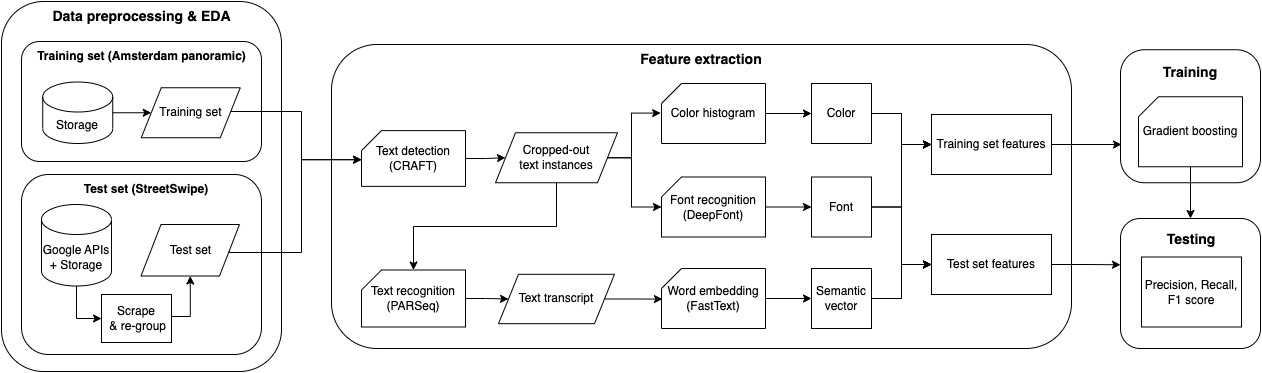
\includegraphics[width=\textwidth]{media/methodology/Pipeline.jpg}
    \caption{Pipeline: Images of facades labelled gentrified or non-gentrified are first fed into the text detection model to extract text instances. Subsequently, the text fonts are extracted with the font classifier, and color histograms are made to record the colors present in each text instances. Text strings are extracted with the text recognition model, before being converted into a vector embedding. \textbf{\textit{[A binary classifier]}} is trained and tested on these 3 features, to classify gentrified facades.}
    \label{fig:pipeline}
\end{figure*}

\subsection{Data}
\subsubsection{StreetSwipe}
The dataset with gentrified and non-gentrified labels is retrieved from the StreetSwipe project \cite{streetswipe}. Using crowd-sourcing, the project let people decide whether each Amsterdam facade is gentrified, by voting "Yes" or "No" on the street view images of these facades. The official \textit{Gentrified} and \textit{Non-gentrified} labels are based on what the majority of people voted for, for each facade. Additionally, if subsequent voters decide against the majority (e.g. voting \textit{Gentrified} for a non-gentrified-labelled facade), they are also prompted to provide a textual reasoning for their decision. These mismatch responses are also available, however is out of scope of the study. 

Since there are two versions of StreetSwipe, the data retrieved exists in two sets, consisting of 1912 higher resolution images from the older version and 529 lower resolution images from the new one. The StreetSwipe dataset thus have 2,441 images in total, each with its numbers of "Yes" and "No" votes, and metadata on the facade's location (latitude and longitude) and street name. The new version's images also have more detailed address, name and type of business/services. There are also more votes in the new version than in the older version. The images from the old version are available directly, while the new ones were provided via URLs to a Google APIs bucket, and thus were scraped.

Feature engineering was done to create the gentrified/non-gentrified label per image, by taking the vote with higher number ("Yes" for gentrified, "No" for non-gentrified). The images were then re-grouped per their corresponding label. Figure \ref{fig:class_size_SS} shows the sample size per class. There is class imbalance in the data, with more than 70\% of the images labelled non-gentrified. This is accounted for in evaluation by using appropriate metrics for classification performance.

\begin{figure}[H]
    \centering
    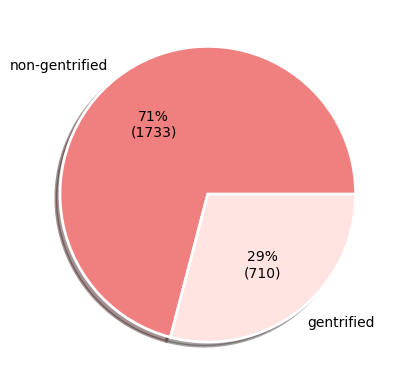
\includegraphics[width=0.4\textwidth]{media/methodology/SS_class_size.png}
    \caption{Sample size per class in StreetSwipe.}
    \label{fig:SS_class_size}
\end{figure}

\begin{figure}[H]
    \centering
    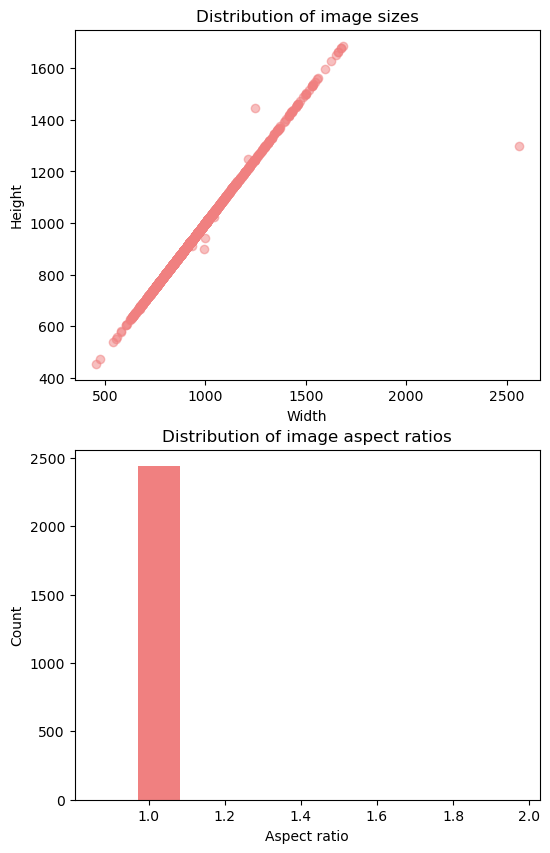
\includegraphics[width=0.35\textwidth]{media/methodology/SS_size_ar.png}
    \caption{Image sizes and aspect ratio distribution in StreetSwipe.}
    \label{fig:SS_size_ar}
\end{figure}

Figure \ref{fig:SS_size_ar} shows that the images have quite consistent aspect ratios of approximately 1:1; however, they vary in size, ranging from around 300x300 to 1700x1700, with one outlier of size 2500x1300 (approximately). No normalization was done at this stage, as the text detection framework does not require a specific image size.

While this dataset contains valuable information - that is crowd-sourced label on gentrification - its size is sub-optimal for training a machine learning model. Therefore, it is used as the test set for the classifier, and another, larger data is used for training.

\subsubsection{Amsterdam street view data}


\subsection{Experimental setup}
\subsubsection{Scene-text detection - CRAFT}
Detecting text in an image, by creating bounding boxes using CRAFT (Character-Region Awareness For Text detection). Compared to another state-of-the-art text detection model - EAST (Efficient and accurate scene text detector) - CRAFT is more accurate and is multi-lingual.

\subsubsection{Scene-text recognition - PARSeq}
Transcribe the image-text into text strings readable by models.

\subsubsection{Color detection}
Create color histograms for the distribution of colors present in the text box.

\subsubsection{Typeface recognition - DeepFont} 

\subsubsection{Semantic analysis - FastText}
Transform the extracted texts into a word vector representation using FastText, to recognize languages and semantics such as cryptic or literal store names, inclusion of ethnicity, religions, etc.

\subsection{Evaluation}
Evaluation is done with the goal to see how accurate the models for extracting fonts, colors, and semantic are. For font and color, this is aimed to be done with the Ma et al.'s synthetic data, with an 80-20 split for the train and test set, respectively. It is appropriate as it has ground truth labels for font and color of text, whereby precision and recall will be calculated. As for the word embedding model, since this is unsupervised, evaluation will be done by examining the word vector's nearest neighbors to see the semantic information the vector captured.